\section{Test case generation via Dynamic Symbolic Execution for Residual Investigation}

\subsection{Introduction and Motivation}

In our evaluation of residual investigation, we can only confirm or down-play 43 bugs out of 436 FindBugs reports. This is largely because native test suites are sparse: many program paths have not been exercised by the native test suite. One might hope we can write additional test cases to augment native test suites. But writing test cases manually is cumbersome and time-consuming. We thus propose to integrate residual investigation with automated test-generation techniques like dynamic symbolic execution (also called ``concolic'' testing).
% In particular, we focus on generating system tests. Generated unit tests may not be realistic; generated system tests attract less debate about the realism of the test cases, because users can see how the tests are used on the client side.  

 %% YANNIS: Throughout the dissertation, you should enforce consistent
 %% naming of the term ``dynamic symbolic execution''. Is it with a
 %% dash (``dynamic-symbolic'') or not? Right now it's mixed. In the
 %% main file it is more often with a dash, but many times without. In
 %% this file, it seems to be without.
Exploiting dynamic symbolic execution is challenging with today's dynamic symbolic execution tools, since tools often fail to generate sequences of method calls to construct desired object states \cite{Xiao:2011:PIP:1985793.1985876}.
% (2) tools cannot reason about the code (e.g. source code or bytecode) of external libraries such as native system libraries and pre-compiled libraries .
% The challenge of using dynamic symbolic execution to generate test cases is that existing dynamic symbolic execution engines are not powerful enough to deal with complicated real-world code (e.g., existing tools cannot generate sequences of method calls to construct desired object states)\cite{Xiao:2011:PIP:1985793.1985876}.  
 We argue that addressing this challenge will require tapping into native test suites to \emph{synthesize new} test cases. The synthesized test cases consist of states (i.e., assignments to variables) induced by native test cases and assignments to some variables that are key to triggering a dynamic condition of residual investigation.  
% The approximate new system tests are not system tests.  They are unit tests with some system state attached.  They are justified by existing system tests so that the unit tests can connect with some execution path tracing back all the way up to program entry (i.e., the main function).  
 We cannot guarantee the realness of such synthesized test cases. It is likely that the argument assignments in the unit tests violate the code's precondition or contradict the states with which we pair the unit tests.  

To see the core ideas and concepts of our test case generation design, consider its application to the program fragment below

\begin{lstlisting}[style=JavaStyle, caption=Simple example program fragment, label=lst:example, frame=none]
class Example {
	main() {
	   A a = ...
	   v = ...
	   a.foo(v);
	}
}

class A {
	B b;
	A(B b) {
		this.b = b;
	}

	foo(v) {
	  bar(v2);
	  baz(v3);
	}

	bar (x) {
	  b.foobar(x2);
	  b.foobaz(x3);
	}

	baz(y) {
	  b.foobaz(..);
	}
}

class B {
	foobar(x) {
	  …
	}

	foobaz(...) {
	  …
	}
}
\end{lstlisting}
 %% YANNIS: What are v2, v3, x2, x3? The example should make some
 %% sense (e.g., refer to defined variables), otherwise is it really
 %% minimal? It should be the bare minimum needed to illustrate the
 %% idea you want illustrated.

Our test case generation design is based on the concept of the call graph: a graph with nodes denoting methods/functions, and edges between them denoting a method/function can call the other.  The associated call graph of the example program is shown in Figure~\ref{fig:call-graph-example}.  For instance, the edge from \sv{A.foo} to \sv{A.bar} in the call graph indicates method \sv{A.foo} can call method \sv{A.bar}. 

\begin{figure}[h]
\centering
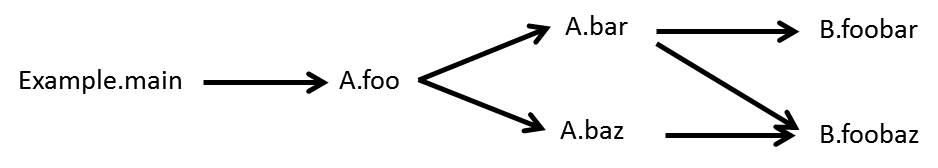
\includegraphics[width=4.0in, trim=0in 0in 0in 0in, clip]{call_graph.jpg}
\caption{The call graph of the example program}
\label{fig:call-graph-example}
\end{figure}

We define a \emph{potential error revealing method (PERM)} as the method that might trigger the dynamic condition of residual investigation for a FindBugs bug pattern.  For example, FindBugs reports an error when a class overrides the \sv{equals(Object)} method but not the \sv{hashCode()} method.  Residual investigation installs a dynamic check for the condition that \sv{Object.hashCode()} is called on an object of the suspect class. The method that contains a call to \sv{hashCode()} on the suspect class (i.e., the class that redefines equals and inherits \sv{hashCode}) or its subclass is the PERM for this bug pattern.  

 %% YANNIS: You abandoned the convention of using \sv{..} for method
 %% names. There should be consistent typesetting throughout. I only
 %% fixed some instances.

%We analyze the PERMs using text search tools like grep, and static analysis techniques such as call graph analysis and Java reflection API.  As an example, for the dropped exception pattern, we analyze the types of the exceptions declared to be thrown by the methods in the suspect code block (suspect methods) using Java reflection and then search for methods whose names are the same as that of any suspect method and throw the same exceptions using grep.  Suppose the method foobar in the above code example is our PERM.  

Once identifying a PERM, we trace $k$ levels back in the call graph from a PERM and call this a switching method.  Returning to our running example, suppose $k = 1$ and \sv{foobar} is a PERM, the method \sv{bar} is a switching method.  

Next we instrument the program under test to record heap state during native test suite execution. The goal of heap state is to provide this object of a switch method call during dynamic symbolic execution (which, recall, often fails to generate sequences of method calls to construct desired object states). The heap state is packed into serialized object files in disk. The kinds of the heap state that we collect include 1) the receiver object on which a switch method is called, 2) the receiver objects on which methods defined in the same class of the switch method are called, and 3) objects that may be used as constructor parameters to initialize the receiver object of the switching method. We use the second kind of heap state to approximate this object of a switch method call when the first kind of heap state are not recorded during the execution of a native test suite from the code under test. In this case, this object of the switch method call is replaced with this objects of other method calls belonging to the same class.  Likewise, we use the third kind of heap state when both the first and second kinds heap states are not recorded. In this case, this object of the switch method call is created by a constructor call using recorded data members.  When some of the data members requires by the constructor call may not be recorded, we use default values (e.g. a reference is assigned null and an integer is assigned \sv{0}).  

\begin{lstlisting}[style=JavaStyle, caption=An example Pig Latin program, label=lst:exampleInstrument, frame=none]

class Example {
	main() {
	   A a = 
	   v = …
	   a.foo(v);
	}
}

class A {
	B b;
	A(B b) {
		this.b = b;
	}

	foo(v) {
	  ObjectWriter.write(this);
	  bar(v2);
	  baz(v3);
	}

	bar (x) {
	  ObjectWriter.write(this);
	  b.foobar(x2);
	  b.foobaz(x3);
	}

	baz(y) {
	  ObjectWriter.write(this);
	  b.foobaz(..);
	}
}

class B {
	foobar(x) {
	  ObjectWriter.write(this);
	  …
	}

	foobaz(...) {
	  ObjectWriter.write(this);
	  …
	}
}
\end{lstlisting}


The resulting instrumented code is run with native tests to collect heap state.

  When hitting a switching method, we start exploring (i.e. switching to dynamic symbolic execution mode, instead of just dynamic execution).  To allow exploration, I relax (i.e., forget) some concrete values.  The first cut is to forget the arguments of switching methods.  In short, the invocation of a switching method turns on dynamic symbolic execution mode during the execution of an existing system test.  I declare victory when I find an approximate system test that calls the PERM method: the unit test case for bar that invokes foobar during its execution given the relaxed state.  In our example, this corresponds to a path like 

\begin{figure}[h]
\centering
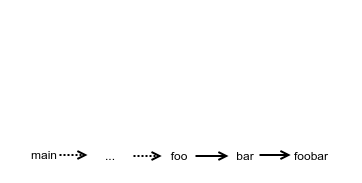
\includegraphics[width=3in, trim=0in 0in 0in 2.0in, clip]{path.png}
\caption{The path that calls the PERM method in the example program}
\end{figure}

The dotted line arrow marks the path before I start dynamic symbolic exploration (i.e. the path exercised by the existing system test), while the solid line arrow marks the path that the generated unit test case for bar establishes. 

PERM definitions for other bug patterns not described earlier:
\begin{itemize}
\item Dropped Exception (DE): FindBugs statically detects dropped exceptions and reports them.  Residual investigation examines which methods end up being dynamically invoked in the suspect code block and watches whether the same methods ever throw the dropped exception when called from anywhere in the program. The methods that contain calls to a method that can be invoked in the suspect code block and can throw exceptions are the PERMs for this bug pattern. 
\item Bad Covariant Definition of Equals (Eq): FindBugs detects that programmers write equals method that accept a parameter of type other than Object.  Residual investigation checks whether the ancestral equals method, Object.equals(Object), is called on an instance of a class that has a covariant definition of equals.  The PERM for this bug pattern is the method that contains a call to equals() on the suspect class (i.e. the class redefines equals and inherits hashCode) or its subclass.
\item Cloneable Not Implemented Correctly (CN): This bug pattern does not require native test suite.  Thus, I do not need to improve existing test suite.
\item Equals Method Overrides Equals in Super-class and May not Be Symmetric 
(EQ\_OVERRIDING\_EQUALS\_NOT\_SYMMETRIC): FindBugs detects whether both the overriding equals method in the subclass and the overridden equals method in the superclass use instanceof in the determination of whether two objects are equal.  Residual investigation dynamically calls both equals method whenever it observes a comparison involving a contentious object and test if the results match.  The PERM for this bug pattern is the method that contains a call to equals() on the suspect superclass or subclass.
\item Non-Short-Circuit Boolean Operator (NS): FindBugs issues warnings for use of \sv{\&} and \sv{|} inside the condition of an if statement.  Residual investigation checks for actual side-effects on the right-hand side of a non-short-circuiting boolean operator.  The PERM for this bug pattern is the method that contains a \sv{\&} or \sv{|} in an if statement.
\item Read Return Should be Checked (RR): FindBugs checks if the return value from read in java.io.InputStream is ignored.  Residual investigation waits until it sees a read method on an object of any subclass of InputStream returns fewer bytes than requested (even for a call that does check the return value).  The PERM for this bug pattern is the method that contains a call to read on the suspect class.
\end{itemize}

\begin{figure*}[htb]
\begin{center}
\begin{scriptsize}
\begin{tabular}{|l|l||c|c|c||}
\hline
\textbf{\#} & \textbf{Instance Method} & \textbf{Branches} & \textbf{Plain Dsc}& \textbf{Dsc+ Serialize} \\
\hline
\hline
1 & \emph{org.apache.bcel.classfile.AnnotationElementValue.dump}	&1&1 & 1 \\ %% 2
\hline
2 & \emph{org.apache.bcel.classfile.AnnotationEntry.dump}	&	2 & 1 & 2 \\ %% 2
\hline
3 & \emph{org.apache.bcel.classfile.Code.accept}	&1 & 0 & 1 \\ %% 3
\hline
4 &\emph{org.apache.bcel.generic.BranchHandle.setInstruction}	& 2 & 1 &2\\ %% 4
\hline
5 &\emph{org.apache.bcel.classfile.ConstantPool.getConstant(index)}	& 2 & 1 &2\\ %% 5
\hline
6 &\emph{org.apache.bcel.classfile.ConstantPool.getConstant(int, byte)}& 4 & 1 &4\\ %% 6
\hline
7 &\emph{org.apache.bcel.generic.ClassGen.addEmptyConstructor}& 1 & 0 &1\\ %% 7
\hline
8 & \emph{org.apache.bcel.generic.ClassGen.removeField}	&1 & 0 &1\\ %% 8
\hline
9 & \emph{org.apache.bcel.generic.ConstantPoolGen.addClass}	& 2 & error &2\\ %% 9
\hline
10 &	\emph{org.apache.bcel.generic.ConstantPoolGen.addFieldref}	& 2 & error &2\\ %% 10
\hline
11 &	\emph{org.apache.bcel.generic.ConstantPoolGen.addMethodref}	& 2 & 0 &2\\ %% 11
\hline
12 &	\emph{org.apache.bcel.generic.ConstantPoolGen.addNameAndType}	& 2 &error &2\\ %% 12
\hline
13 &	\emph{org.apache.bcel.generic.ConstantPoolGen.addString}	& 2 &error &2\\ %% 13
\hline
14 &	\emph{org.apache.bcel.generic.ConstantPoolGen.addUtf8}	& 2 &error &2\\ %% 14
\hline
15 &	\emph{org.apache.bcel.generic.ConstantPoolGen.lookupClass}	& 2&1 &1\\ %% 15
\hline
16 &	\emph{org.apache.bcel.generic.FieldGenOrMethodGen.removeAttribute}	& 1 & 0 &1\\ %% 16
\hline
17&	\emph{org.apache.bcel.generic.FieldGenOrMethodGen.setType}	& 2 & 2&2\\ %% 17
\hline
18&	\emph{org.apache.bcel.generic.InstructionHandle.addTargeter}	& 1 & 0 &1\\ %% 18
\hline
19&	\emph{org.apache.bcel.generic.InstructionHandle.setInstruction}	& 2 & 0 &2\\ %% 18
\hline
20&	\emph{org.apache.bcel.generic.InstructionList.append}	& 1 &1 &1\\ %% 18
\hline
21 &	\emph{org.apache.bcel.generic.InstructionList.setPositions}	& 2& N/A & 2\\ %% 16
\hline
22 &	\emph{org.apache.bcel.generic.MethodGen.addLocalVariable}	& 3 & 0 &3\\ %% 16
\hline
23 &	\emph{org.apache.bcel.generic.MethodGen.removeCodeAttribute}	& 1& 0 & 1\\ %% 16
\hline
24&	\emph{org.apache.bcel.util.ClassPath.getInputStream(String)}	& 2& 0 & 2\\ %% 16
\hline
25 &	\emph{org.apache.bcel.util.InstructionFinder.search}	& 2 & error & 1\\ %% 16
\hline
26& \emph{org.apache.bcel.util.SyntheticRepository.findClass}	& 2& 1 & 2\\ %% 16
\hline
27 &\emph{org.apache.bcel.util.SyntheticRepository.loadClass}	& error& 1 &1 and then error\\ %% 16
\hline
28 &\emph{org.apache.bcel.util.SyntheticRepository.storeClass}	& 1& 0 & 1\\ %% 16
\hline
\end{tabular}
\caption{Summary of our experiments on the AspectJ Compiler.}
\label{fig:ajc-results}
\end{scriptsize}
\end{center}
\end{figure*}
